\documentclass[tikz,convert={outfile=\jobname.svg}]{standalone}

\usepackage{minted}
\usepackage{tikz}

\begin{document}
\small
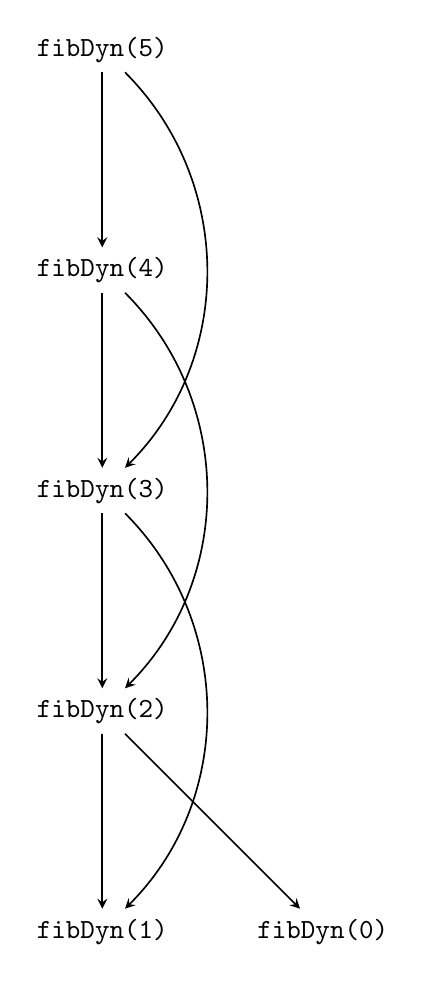
\begin{tikzpicture}[->, >=stealth, auto, node distance=2.8cm, semithick]

    \tikzstyle{state}=[text=black]

    \node[state] (A)  {\texttt{fibDyn(5)}};
    \node[state] (B) [below of=A] {\texttt{fibDyn(4)}};
    \node[state] (C) [below of=B] {\texttt{fibDyn(3)}};
    \node[state] (D) [below of=C] {\texttt{fibDyn(2)}};
    \node[state] (E) [below of=D] {\texttt{fibDyn(1)}};
    \node[state] (F) [right of=E] {\texttt{fibDyn(0)}};

    \path (A) edge (B)
              edge [out=315,in=45] (C)
          (B) edge (C)
              edge [out=315,in=45] (D)
          (C) edge (D)
              edge [out=315,in=45] (E)
          (D) edge (E)
              edge (F);
\end{tikzpicture}
\end{document}